\chapter{Mining User Interface Design Pattern Changes}
\label{ch:mining_design_changes_chapter}
Mobile user interface (UI) design patterns have been widely used across different mobile platforms.
UI design patterns have evolved and changed significantly as new trends emerge and fade at different times.
This chapter presents a data-mining approach to analyzing design pattern changes in Android apps.
Over a period of 18 months, we tracked 24,436 apps and collected their versions.
In total, our sample consists of 56,349 unique app versions, more than 5 million source files, and more than 25 million UI elements.
We developed a dedicated infrastructure based on modern big data technologies to support our differential analyses regarding design pattern changes.

The work presented here is the result of collaboration with Tom Yeh (\cite{Alharbi_2015_MobileHCI}).
\section{Introduction}
UI design patterns are general, reusable solutions to common design problems.
Take, for example, the problem of organizing menu items on a small screen of a mobile device.
A number of design patterns have emerged as useful solutions to this problem.
For instance, Android design guidelines feature a number of design patterns such as the use of ``Navigation Tabs'' pattern \cite{action_bar_nav_tabs} and the ``Navigation Drawer'' pattern \cite{nav_drawer}.
Design patterns are valuable to both third party app developers and UI framework engineers.
UI framework engineers invest a substantial amount of time and effort in building new design patterns for their platforms to enable third-party app developers to enhance the UIs of their applications.
Third-party developers make difficult decisions when choosing a particular design pattern to communicate their ideas in a way that pleases their users.
A good design pattern often enjoys wide adoption by developers and acceptance by users.
An interface following good design patterns is familiar to users, consistent with users' expectations, and easy to learn.
A bad design pattern would have the opposite effects.

\par Design patterns change, evolve, or in some cases, die out over time.
A design pattern once popular may begin to lose popularity to a better alternative. 
A once obsolete pattern may experience a resurgence in adoption.
A new design pattern may be introduced with a lot of hype and promises but never go on to wide adoption.
A little-known design pattern may all of a sudden explode in popularity.
These phenomena may have important HCI implications. But there has not been a large-scale comprehensive study on changes in design patterns.

\par The design guidelines of mobile applications have changed significantly with new design patterns, UI elements, and styles to improve the overall visual design of mobile apps. UI framework engineers add new widgets for complex UIs, implement new APIs for them, deprecate previous widgets and UI related APIs, and add new visual design patterns to help developers build beautiful applications. How do we know how many apps have made the switch to a particular design pattern and maintained the usage across future releases? 
It is hard to quantify the adoption rate of these design patterns using existing approaches.

\par This chapter presents a data-driven approach to studying design pattern changes on a large scale.
We applied this approach to the Android framework and present our findings here. 
Our approach consists of five steps:

\begin{enumerate}[itemsep=0ex,parsep=0ex]
	\item Collect a large number of apps. Continue to download their subsequent updates.
	\item Decompile each app into code that can be analyzed to understand the app's UI design (e.g., XML) and actual programmed behaviors (e.g., void onClick()).
	\item Extract a comprehensive set of features about each app from the app's listing details web page, user interface layout, and actual code.
	\item Stats: Compute statistics (e.g., distribution, min., max, mean, outliers) with respect to a feature of interest.
	\item Diff: Compare two versions of an app and compute their differences. Identify common and unusual change patterns.
\end{enumerate}

\par Our approach provides new insight into design pattern changes in Android apps.
For example, there are five common design patterns for navigation: Tab Layout, Fragments, Horizontal Paging, Up Navigation, and Navigation Drawers.
Which of these are more common?
Have any apps made a switch between two pattern versions?
What are the most common switches? How prevalent are they?
What apps use an unusually large number of custom widgets?
Are there apps switching from custom widgets to built-in widgets? These are just a sample of questions our approach was able to address.

\par We present our approach in detail, describe a system that supports our application of this approach to the Android framework, and finally present eight analyses of design pattern changes to demonstrate the usefulness of our approach.
\section{Approach}

Our approach consists of five steps: collect, decompile, extract, stats, and diff.
We choose the Android platform as an application and explain how we carry out each step to analyze design pattern changes.

\begin{table*}[t]
	\def\arraystretch{2}
	\centering
	\begin{tabular}{|p{2.2cm}|p{13cm}|}
		\hline
		\textbf{Listing \ Details \ Features} &
		package name, title, description, reviews, store URL, category, price, date published, version name, version code, target system version, ratings count, rating, content rating, creator, creator URL, install size, downloads count, permissions, what's new.\\
		\hline
		\textbf{Appearance \ Features} &
		layout directories, layout files, view group containers, view elements, relationships, drawable resources, UI text resources.\\
		\hline
		\textbf{Behavioral \ Features} &
		app framework invocations, manifest (AndroidManifest.xml), third-party libraries.\\
		\hline
	\end{tabular}
	\caption{List of features extracted from each app.}
	\label{tab:table_features}
\end{table*}

\subsection{Collect}
The first step is to collect a large sample of apps and extract the visual structure of their user interfaces.
We download apps from the official marketplace, Google Play store, and crawl their listing details web pages.
Moreover, in order to analyze changes, we need to continue to monitor these apps for updates and download them.

\subsection{Decompile}
The second step is to decompile the user interface program to expose its ``code'' portion so that the actual programmed behaviors can be subject to analysis.
This step involves running an ``unpack'' tool to open each app's Android Application Package (APK) file to obtain a set of design layout files and a ``dissembler'' tool to obtain the app's byte code.

\subsection{Extract}
The third step is to compute a rich set of features to describe each app at three levels.
First, at the listing details level, we find descriptive information about a GUI from where the GUI may be listed, promoted, or reviewed.
Second, at the appearance level, we gather data that defines the look and feel, content, and structure of a GUI.
Third, at the behavioral level, we examine the decompiled code to gain insight into the actual programmed behaviors of a GUI.
We mine the Google Play store to obtain a comprehensive set of listing features, such as the title, price, ratings, install size, and what is new.
We parse the manifest file, the layout files, and the string definition files to extract appearance features such as the use of custom components and the relationships between components.
Finally, we apply program analysis to the byte code to extract the behavioral features such as the use of GUI related APIs that dynamically change the GUI. 
Table~\ref{tab:table_features} gives a comprehensive list of the features we considered on the three levels.

\subsection{Stats}
After extracting a rich set of features about the apps in the corpus, the fourth step is to conduct statistical analysis about them.
The most common analyses would be to compute the average, min, max, and histogram for quantitative features.
For categorical features, counting and distribution often yield useful insights. For text features, one can compute the most frequent words.
Complex analyses are possible at this step, such as correlations, clustering, outliers detection, and sentiment analysis.
In the application of design pattern changes, we carry out a range of statistical analyses like ``what's the percentage of apps using a given design pattern?'' and ``what's the percentage of apps that switch to a different design pattern?''
Although computing descriptive statistics on UI design pattern changes seems simple, it was not even possible before our approach.

\subsection{Diff}
The final step is to compare two subsequent versions of an app and identify the aspects that have been updated.
Usually an update contains changes to certain aspects of an app's GUI design. Sometimes changes are obvious, such as design overhaul.
Sometimes changes are subtle, such as rewording the caption of a button. We pay attention to changes that occur in the listing, the appearance, and the behaviors.
For instance, an app may add a new screen to support a new feature.
This change can be reflected at all levels, including description in the ``what's new'' section promoting the new feature, an extra layout file defining the new screen, and an extra function calls in the app's code to implement the new features.
Moreover, we consider differences at the group level, by asking, for example, what are the most common design patterns dropped in a collection of apps?

\section{System Implementation}

On a small scale, the five steps in our approach are easy to carry out.
But they quickly become challenging when the scale goes up to a level of tens of millions of layout and program files.
There is no off-the-shelf, ready-to-use system to support large-scale differential analyses to answer our questions regarding design pattern changes.
Therefore, we designed and implemented a system dedicated to supporting our analyses. The technical detail of this system is presented here.

\begin{figure*}[!t]
	\centering
	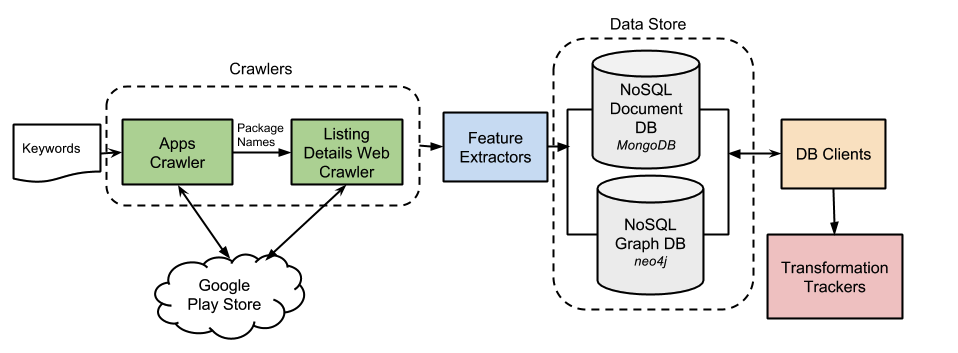
\includegraphics[width=16cm, height=5cm]{figures/design-pattern-changes/system_architecture}
	\caption{Architecture of the analytic system.}
	\label{fig:fig_system_architecture}
\end{figure*}

\begin{table*}[!t]
	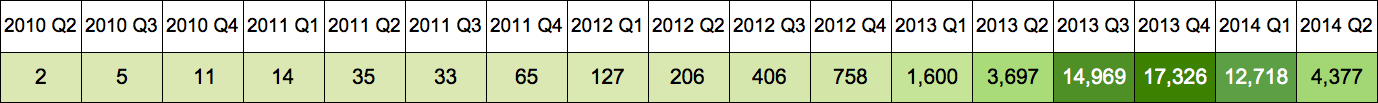
\includegraphics[width=16cm, height=2cm]{figures/design-pattern-changes/release_date}
	\caption{The number of apps by release date grouped by quarters.}
	\label{tbl:release_date}
\end{table*}

\par The system consists of five components (see Figure~\ref{fig:fig_system_architecture}): Apps crawlers, feature extractors, data stores, client drivers, and transformation (changes) trackers.
The apps crawler downloads free apps from the Google Play Store and saves them to the file system.
Feature extractors are a rich tool chain that decodes apps, extracts features, and stores them in the data stores.
The client drivers handle all interaction with the data stores.
The change trackers are a rich tool chain that tracks and computes statistics on changes to the extracted features.

\subsection{Apps Crawlers}
Our system utilizes two custom crawlers we built: the apps crawler and the listing details web crawler.
The apps crawler maintains a list of keywords, crawls the Google Play Store, and returns a list of package names for free apps.
We used Google-Play-Crawler \footnote{http://github.com/Akdeniz/google-play-crawler}, an unofficial open-source Java API for the Google Play Store, to retrieve package names and download APK files.
Prior releases of apps are not available on the Google Play Store.
Thus, the apps crawler obtains the version code value for each retrieved package name and queries the data store to check if it exists.
If it does not already exist in the repository, the crawler downloads and saves the APK file in the data store.

\par Once the APK file is downloaded, the apps crawler notifies the listing details web crawler to download the most recent app listing details web page.
The listing details web crawler is written in Ruby.
It generates a URL using the package name and downloads both the HTML page and the resources of the listing details web page.
Finally, another process runs to decode the APK file using Apktool \cite{apktool}, an open-source reverse-engineering tool.
When the APK file is decoded, we get a directory tree of app files that make up the app.

\subsection{Feature Extractors}
Once an APK file and its listing details web page have been downloaded, a set of feature extractors is run.
The feature extractors comprise three main tools: Listing details extractor, UI extractor, and source code extractor.
The listing details extractor parses the listing details HTML file, extracts the features, and stores them in the document data store.
The UI extractor traverses the unpacked APK file, extracts UI features from layout files and resources, and stores them in the graph data store.
The source code extractor computes features from the smali files, a human readable assembly like language for the disassembled byte code.
It uses string pattern matching techniques (e.g., grep, regular expressions) to extract features available in the app's byte code and stores them in the document data store.

\subsection{Data Stores}
Our data store is built on top of two database technologies: a NoSQL document-oriented database for storing apps listing detail features, code features, and APK files.
The second database is a graph database for storing the XML elements of layout files. The document-oriented database is a MongoDB instance, an open-source document- oriented database scalable to accommodate large and complex data. Our MongoDB instance comprises five collections: listing details, the AndroidManifest features, code features, and two GridFS collections to store the binary APK files and additional metadata. The MongoDB instance contains collections for over 56,349 APK files for 24,436 unique apps with multiple releases. The total size of the database is 501 GB hosted on a 24-core server with 47 GB RAM running Ubuntu 12.04. Over the observation period of our analysis (from January 2013 to June 2014), we collected a minimum number of versions per app in two versions in our dataset, which represents 80.1\% of the dataset (Figure~\ref{fig:fig_dataset}). Table~\ref{tbl:release_date} shows the number of apps by release date, and Figure~\ref{fig:fig_downloads_ratings} shows the download count distribution by their ratings.
\begin{figure}
	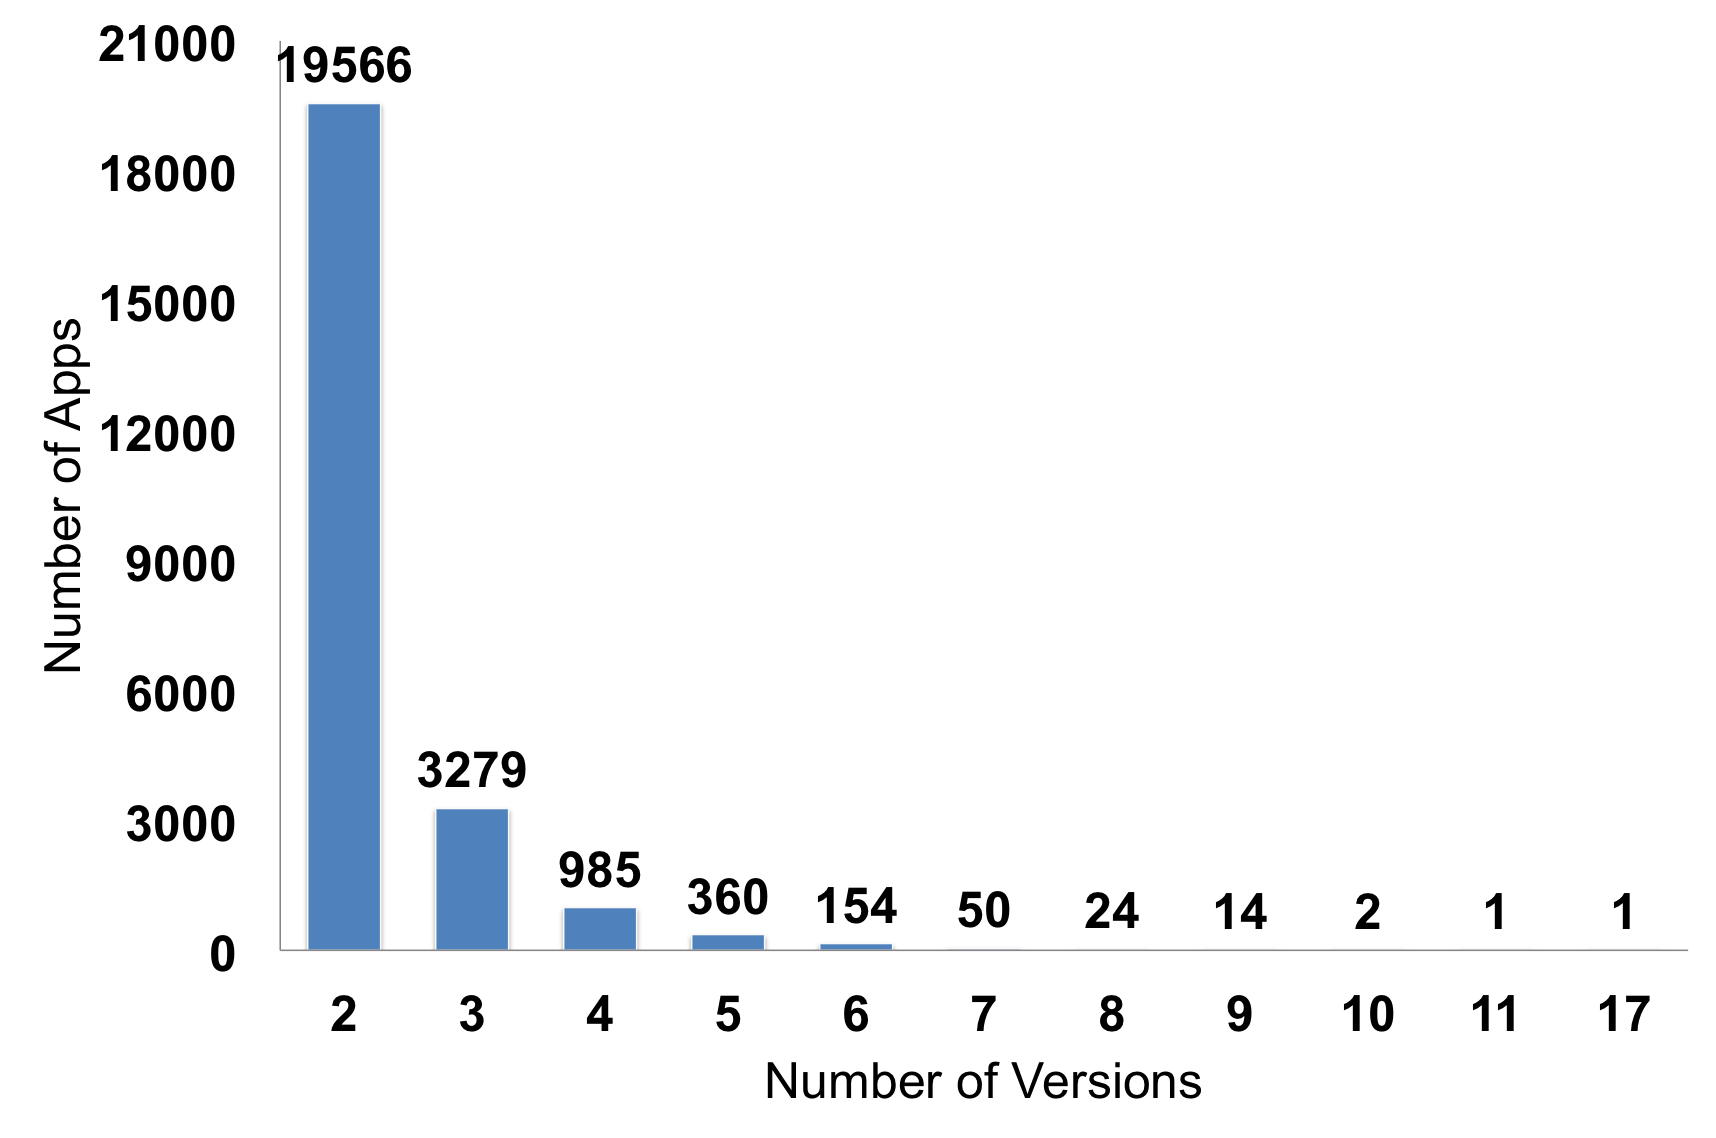
\includegraphics[width=6in, height=3in]{figures/design-pattern-changes/dataset}
	\caption{The distribution of apps by versions.}
	\label{fig:fig_dataset}
\end{figure}


\begin{figure*}[!t]
	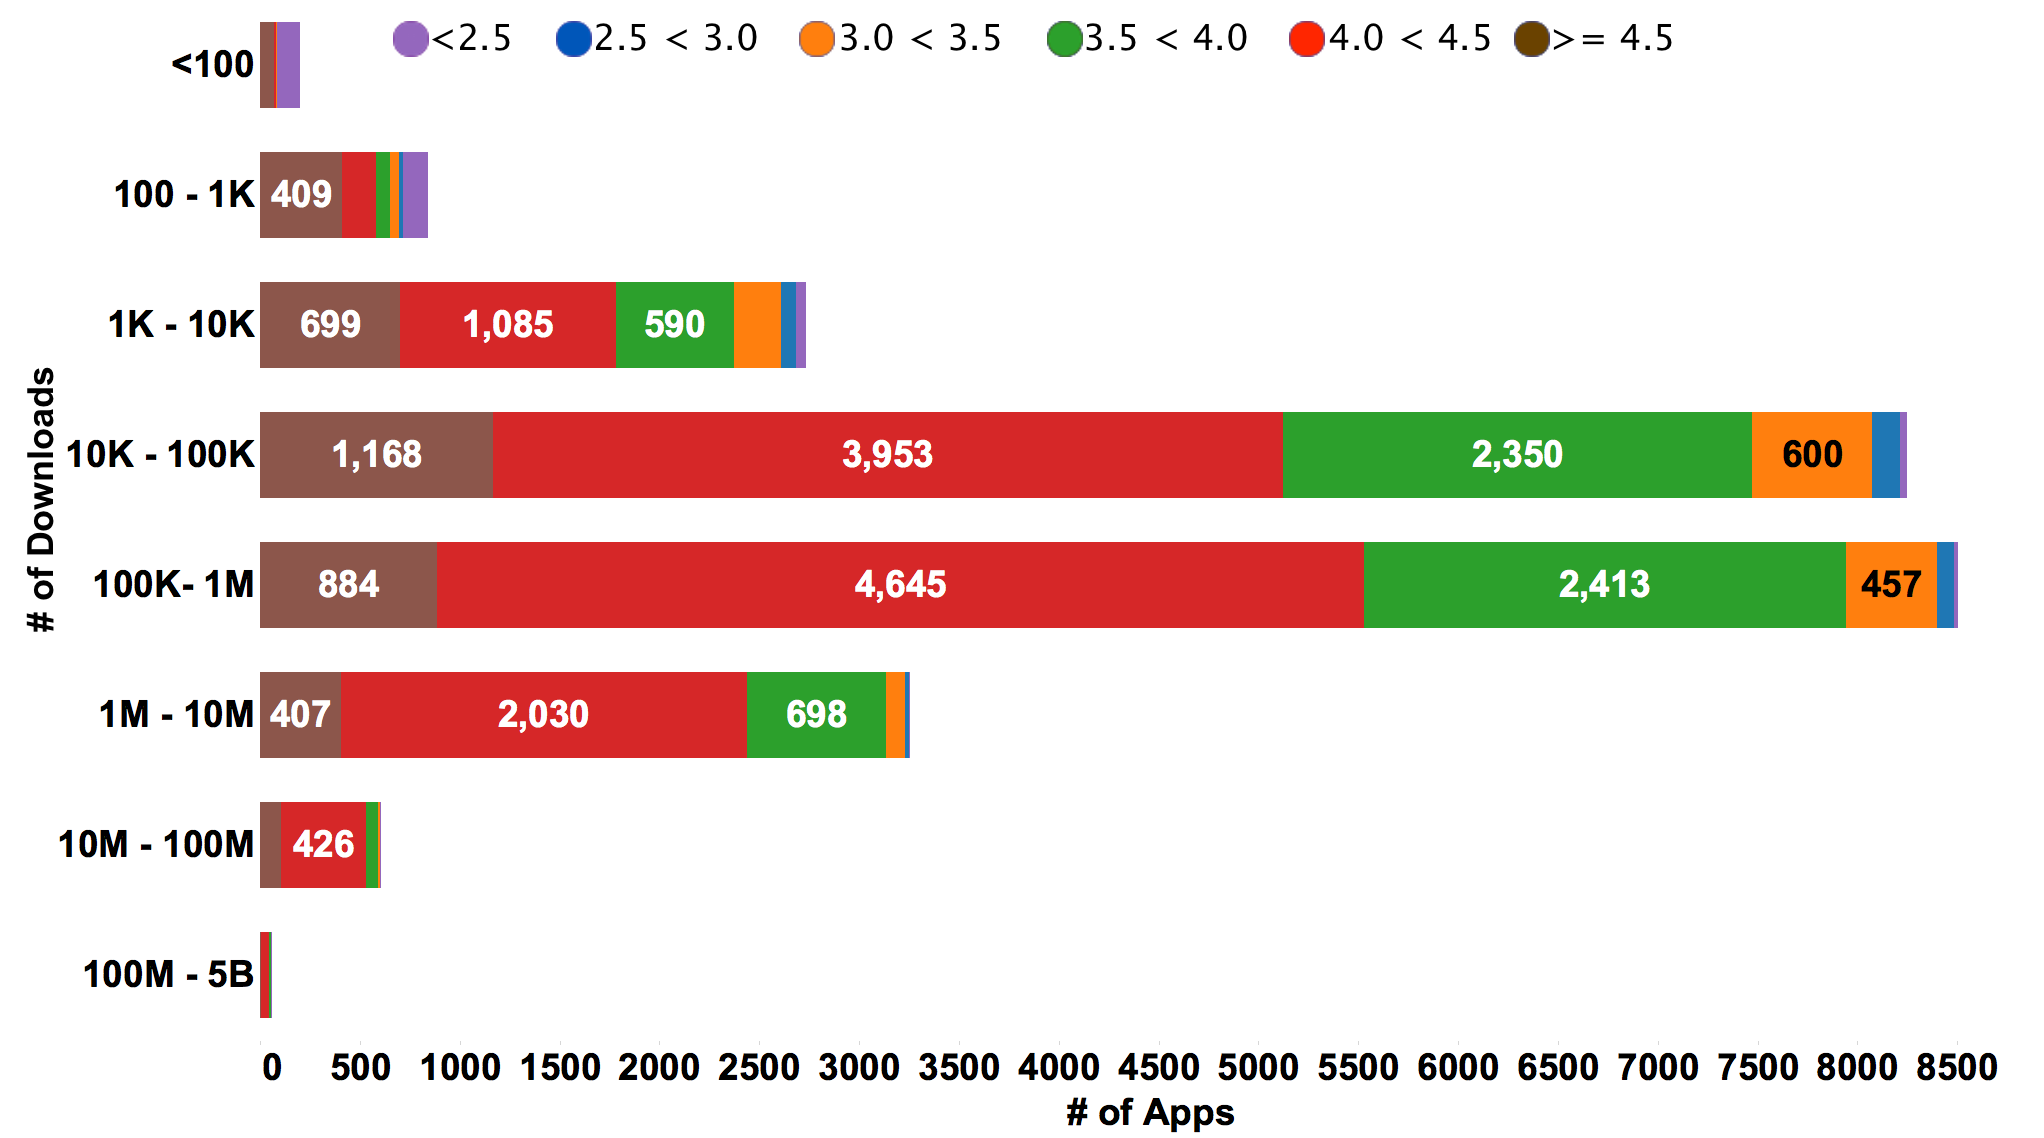
\includegraphics[width=16.5cm, height=8cm]{figures/design-pattern-changes/downloads_ratings}
	\caption{The download distribution of the apps by rating stars. Colors show details about the rating.}
	\label{fig:fig_downloads_ratings}
\end{figure*}

\par
The graph database is a Neo4j server. Graph databases are well suited to model hierarchical connected data like UI structure.
Neo4j uses the property-graph model, which allows storing XML elements with their attributes (key-value-pairs) in graph nodes.
In android, developers can reuse multiple layouts using the ``\textless include \textgreater '' tag to embed layouts to the current element in the hierarchy.
Our UI feature extractors attach the included layout to the current UI tree element, connecting layouts to one app tree.
Queries like ``find a specific ViewGroup element with two specific children'' run faster than the traditional many JOIN queries in Relational DBs.
In our database model, each UI element (e.g., a view like ImageView or a view group 
like LinearLayout) corresponds to a graph node connected with one relationship (e.g., has view, has view group).
The number of graph nodes in our database is 29,733,591 nodes.

\subsection{Database Client Drivers}
A set of MongoDB drivers is running to query and retrieve data from the database.
The complexity of the executed queries varies from finding fields in multiple collections to running multiple-pass mapReduce tasks.
The graph database clients execute transaction queries on the graph database using Cypher language, a graph query language for querying Neo4j graphs.
These clients output the results as CSV files to be processed by the transformation trackers.

\subsection{Transformation Trackers}

To interpret the results generated by the client drivers, another set of tools are running to compute statistics on the generated results.
These are data analysis tools written in Python using the Pandas library, an open-source library for high-performance data analysis.
The data store client drivers output the results as CSV files, which are passed as input to the transformation trackers.
The transformation trackers load each CSV file into a Data Frame, a tabular data structure with labeled axes.
The Data Frame is indexed by an array of tuples where each tuple is a unique value of the app's package name and version code values.
This makes it easier to track changes and perform sophisticated data analysis on multiple versions.

\section{Design Pattern Changes}
The system we developed has enabled us to conduct many analyses on design pattern changes.
Here we chose eight of the most illustrative ones to present: custom UI components, home screen widgets, as well as various ways of navigating: Tab Layouts, Fragments, Horizontal Paging, Action Bar with Tabs, Up Navigation, and Navigation Drawers. 
For each analysis, we discuss the motivation, method, results, and implications.

\subsection{Custom UI Components}

\subsubsection{Motivation}

A GUI framework typically provides a rich set of standard UI widget classes with the goal to ease the GUI development effort.
Developers often can meet their needs using these widget classes. 
If not, they may need to define custom UI widget classes. 
Some custom components are provided by third-party libraries to provide custom widgets or backward-compatibility of the standard components. 
Others are developer-customized components. 
How prevalent is the use of custom widgets? We are interested in this question because extensive uses of custom widgets may be a sign that the standard UI widget classes are inadequate.
\subsubsection{Method}
A custom component is declared in layout files using the full qualified class name of the component's class file which starts with a package name, such as
\begin{minted}{xml}
<com.android.notepad.MyEditText id="@+id/note" />
\end{minted}
rather than using the name of one of the default widget classes such as EditText, TextView, and Button.
Thus, to find evidence of use of custom UI components in an app, we queried the graph database for apps with views that start with a package name and counted the number of declarations of this form in all of the app's layout files.

\subsubsection{Results}

We found 15,808 (64.7\%) apps used at least one custom component, which is more than half of the apps in our corpus. 
Among them, 818 (5.2\%) apps initially did not use any custom component and began using it after an update. 
410 (2.6\%) apps did the opposite, reverting to use only standard components in subsequent updates. 
We looked at the listing details of these apps to find if the developers described any information related to this change in the listing details section ``What's New''.
We searched for UI related keywords and discovered apps that report enhancements to tablets and large screens.
For example, one app stated, ``App is optimized for tablets and many UI enhancements'' and another app stated ``Improved layout and graphics for larger screen''.
We also looked for unusual change patterns.
For example, we were interested in whether there were apps that had introduced a large number of custom components after an update.
We found 58 apps added more than 500 custom components after updates. 
We identified  234 unique custom components in these apps by the first three parts of the custom component name (e.g., com.airbnb.android).
The top three added custom libraries are: android.support.v4 (18.8\%), com.facebook.widget (11.5\%), and com.actionbarsherlock (5.1\%).
Interestingly, we observed a high concentration of these apps in the Finance category.
To dig further, we examined the ``what's new'' section of these apps and found mentions of ``tablets'' and ``large screens'' that coincide with this sudden increase in the use of custom components.
For example, one app stated ``Accept payment on Tablets'' and another one stated ``Resolved login crashes on multiple Tablets.''

\subsubsection{Discussion}

Even though most of the standard Android UI components provide built-in support for automatic scaling to fit content on large screens, getting these components to work properly may require a tremendous amount of effort by developers.
We speculate that the 818 (5.2\%) apps we found that had begun to use custom components may be to achieve better large screen support that is not offered by standard components.
We found there were more apps adding custom components than those removing custom components.
This suggests an increased level of reliance on custom components over our sample of Android apps.
One could interpret this as a sign that default components are gradually becoming inadequate.

\subsection{Home Screen Widgets}

\subsubsection{Motivation}

Home screen widgets are shown on the user's home screen to provide immediate access to useful information (e.g., today's weather) or control of commonly used functionalities (skipping to the next song).
By choosing which app's home screen widget to display, a user may implicitly indicate her preference for the app. 
Since there is limited area on the home screen, the size of a home screen widget matters. 
An app widget may provide a set of predefined dimensions (e.g., 1x1 or 2x2). 
Some apps may allow the users to adjust or stretch the dimensions of its home screen widgets freely.

\subsubsection{Method}

To find apps that use widgets, we queried the document database for apps that declare widgets in the app’s AndroidManifest.xml file. 
In this file, the \textit{\textless receiver\textgreater} element has a child element named \textit{\textless meta-data\textgreater} that has an attribute named \textit{android:name} whose value is set to \textit{``android.appwidget.provider''}. 
To support resizable widgets, Android developers need to declare the resize mode to be horizontal, vertical, or both by setting the value of the attribute \textit{resizeMode} of the \textit{\textless appwidget-provider\textgreater} element located at \textit{res/xml/}. 
To find resizable widgets, we queried the UI graph database to a find a widget layout file whose root element is \textit{\textless appwidget-provider\textgreater} with the attribute \textit{resizeMode}.

\subsubsection{Results}

We found 2,639 apps (10.8\%) support home widgets.
Among them, 255 (9.6\%) added home widgets for the first time, and 80 (3\%) later dropped home widgets altogether. 
1,118 (42\%) apps allow home widgets to be resizable. 
Among these, 295 (26.4\%) were not resizable before and became resizable only in the most recent release. 
24 (2.1\%) apps had resizable home screen widgets but later on disabled the resizing functionality. 
In all cases, we did not find any information in the listing (i.e., description and what's new sections) mentioning changes in home widget support. Figure~\ref{fig:fig_resizble_widgets}
\begin{figure}[!t]
	\centering
	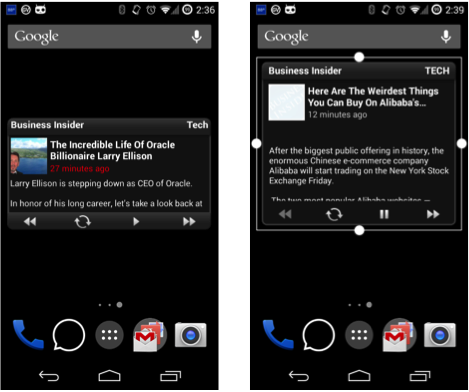
\includegraphics{figures/design-pattern-changes/resizble_widgets}
	\caption{Two versions of an app titled ``Business Insider'' before (left) and after (right) adding the resizing functionality to its home screen widget.}
	\label{fig:fig_resizble_widgets}
\end{figure}
shows an example of a home screen widget of an app before and after making it resizable.

\subsubsection{Discussion}

We found more apps adding support for home screen widgets than those dropping the support (255 vs. 80). 
This suggests an increased adoption of home screen design pattern. 
Among those already providing home screen widgets, a similar trend of increased adoption of the ``resizable'' pattern is observed. 
This suggests apps are increasingly competing for the limited home screen space. 
Apps that did not provide home screen widgets would lose out because users are unable to place them on their home screen and may use them less frequently as a result.

\subsection{Tab Layout with TabHost}

\subsubsection{Motivation}
Tab layouts are used to hold a set of tab labels to allow users to navigate between different content. 
One way to implement this design pattern is through the TabHost API. 
We chose this API for two reasons. 
First, this API was included in the initial release of the Android GUI framework (level 1). 
Second, it was later deprecated (level 11) in favor of new navigation patterns, such as the Fragment and the Action Bar patterns. 
We were interested in whether most or only a small percentage of apps had made this transition.

\subsubsection{Method}
In order to create a tabbed UI, developers need to use a ViewGroup element named TabHost and a View element named TabWidget. 
We queried the UI database for a GroupView named TabHost with a child View named TabWidget.
\subsubsection{Results}
We found 3,809 (15.6\%) apps used TabHost in their UIs. 
Among them, 666 (17.5\%) apps used TabHost for the first time and 413 (10.8\%) apps stopped using it and shifted to other types of navigations. 
We further inspected their listing details to see if it includes reasons that describe the migration. 
We found 106 (25.58\%) of these apps provided explanations in their listings. 
DDLive is an example of an app that has undergone this change. 
In the ``what's new'' section of its listing on Google Play, the phrase ``UI Changes for better experience'' can be found. 
Figure~\ref{fig:fig_tabhost}
\begin{figure}[!t]
	\centering
	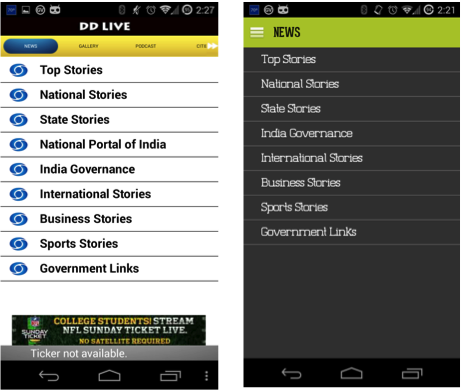
\includegraphics{figures/design-pattern-changes/tabhost}
	\caption{Two versions of an app titled ``DDLive''. The version on the left uses TabHost and the version on the right uses a Fragment that contains a list of items.}
	\label{fig:fig_tabhost}
\end{figure}
shows two screenshots of the app before and after the migration from the TabHost pattern to the Fragment pattern.

\subsubsection{Discussion}
The migration rate of this design pattern is very slow. 
Even though the TabHost pattern has been deprecated for at least three years, some new apps continued to use it. 
Existing apps using them slowly dropped the use of the TabHost pattern but not at a very fast rate. 
This raises the question of why deprecated APIs and design patterns enabled by them are so ``sticky'' among Android apps.

\subsection{Fragment}

\subsubsection{Motivation}
Fragments are used to create a multi-pane view and a responsive UI that works on a variety of screen sizes and devices. 
It is a relatively new design pattern that was introduced in API level 11 to allow developers to add multiple independent UI components and reuse them in different parts of the UI with its own lifecycle. 
We were interested in how widely this design pattern was adopted.

\subsubsection{Method}
Fragments can be statically added to the layout files or dynamically added in the source code. 
Thus, our analysis needs to look at both the UI and code. 
In the UI, we query the UI database for apps with the \textit{\textless fragment \textgreater} element and obtain the value of the \textit{android:name} attribute that references a class in the source code. 
In the code, we search for the class to see if it extends the Fragment class or any of its subclasses.

\subsubsection{Results}
We found 3,963 (16.2\%) apps used the Fragments pattern. 
Among them, 1,814 (45.8\%) used Fragment for the first time and only 139 (3.5\%) apps stopped using it in recent releases. 
Figure~\ref{fig:fig_fragment}
\begin{figure}[!t]
	\centering
	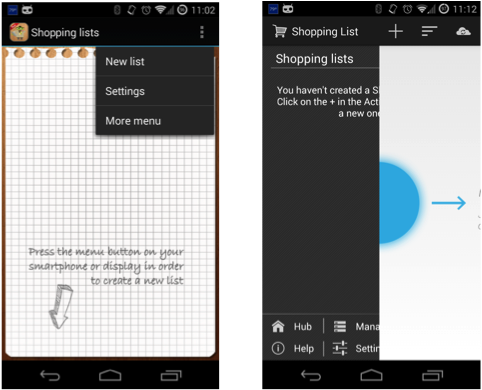
\includegraphics{figures/design-pattern-changes/fragment}
	\caption{Two versions of an app titled ``Shopping List'' before (left) and after (right) adopting the Fragment design pattern.}
	\label{fig:fig_fragment}
\end{figure}
shows an example of a shopping list app before and after using Fragment pattern.

\subsubsection{Discussion}
It had been four years since the Fragment pattern was introduced. 
We initially anticipated to observe a broad adoption of the Fragment pattern by apps to take advantage of the benefit this pattern offers. 
We instead found a lower than expected adoption rate. 
Only 3,963 (16.2\%) of the apps use it. 
Among them, almost half were recent adoption during our observation period. 
We speculate that the Fragment pattern is a lot more complicated to implement. 
For example,  StackOverflow, a popular online community for developers to ask and answer questions about coding, has over 16,100 questions tagged with ``android-fragments''. 
Some developers may rather stick to what they are familiar with rather than risking implementing the switch to the Fragment pattern incorrectly.

\subsection{Horizontal Paging}

\subsubsection{Motivation}
Horizontal paging is a navigation pattern that allows users to navigate between screens using left and right swipes. 
We explore this design pattern to find how wide this type of interaction is and how preferable it is over multiple releases.
\\
\subsubsection{Method}
To implement this pattern, the most common approach is to use a \textit{ViewPager} view group, which is a container that can hold multiple child view elements, each of which represents a distinct screen. 
Child views can be populated using \textit{PagerAdapters} in the source code. 
To find apps with this pattern, we queried the UI graph database for apps that use the \textit{ViewPager} element as a \textit{ViewGroup} container and make use of any \textit{PagerAdapters} subclasses in the source code.

\subsubsection{Results}
We found 4,524 (18.51\%) apps used the Horizontal Paging pattern. 
Among them, 941 (20.8\%) added this pattern for the first time. 149 (3.3\%) apps dropped this pattern. 
Figure~\ref{fig:fig_horizontal_paging}
\begin{figure}[!t]
	\centering
	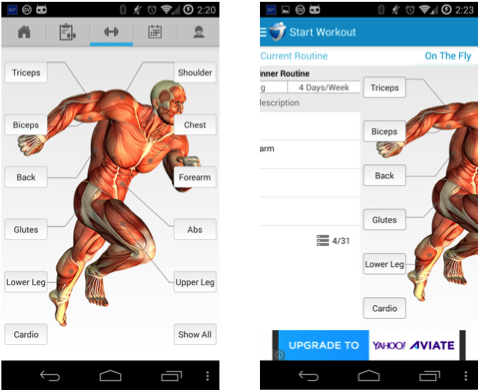
\includegraphics{figures/design-pattern-changes/horizontalpaging}
	\caption{Example of an app titled ``JEFIT Workout Exercise Trainer'' before (left) and after (right) adopting the Horizontal Paging design pattern.}
	\label{fig:fig_horizontal_paging}
\end{figure}
shows an example of an app before and after using the horizontal paging design pattern.

\subsubsection{Discussion}
We observed a lower first-time adoption rate of the Horizontal Paging pattern than that of the Fragment pattern. 
This suggests that Horizontal Paging pattern has a longer history than the Fragment pattern. 
Apps still continue to migrate to these two patterns but more of them chose the more general Fragment pattern.

\subsection{Action Bar with Tabs}

\subsubsection{Motivation}
Action Bar provides several functions to an app including the screen title, action buttons, and a navigation view with two modes of navigations: navigation tabs or drop-down lists. 
It was first introduced in Android 3.0 (API level 11) but also available for lower API levels through additional support libraries. 
We explore the use of the Action Bar with navigation tabs, and how apps have maintained the use of this pattern in their recent versions.

\subsubsection{Method}
While there are multiple ways to create an Action Bar with navigation tabs, they all require implementing the \textit{ActionBar.TabListener} interface that provides the required callbacks to respond to user's actions. 
To explore the use of Action Bar with tabs, our analysis needs to look at the code. 
We search the source code for apps that implement the \textit{TabListener} interface.

\subsubsection{Results}
We found 8,483 (34.7\%) apps used the Action Bar with Tabs. 
Among them, 2,729 (32.2\%) were first-time adopters of this pattern. 330 (3.9\%) stopped using it. Figure~\ref{fig:fig_actiobar_tabs}
\begin{figure}[!t]
	\centering
	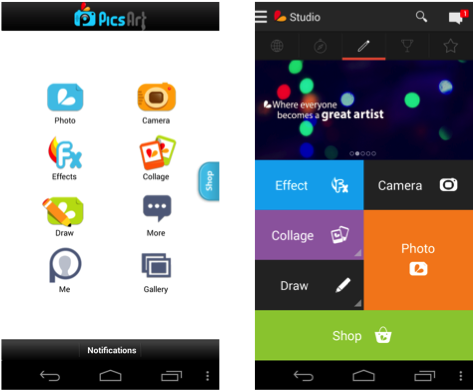
\includegraphics{figures/design-pattern-changes/actiobar_tabs}
	\caption{Two versions of an app titled ``PicsArt'' before (left) and after (right) adopting the Action Bar pattern with Tabs.}
	\label{fig:fig_actiobar_tabs}
\end{figure}
shows an example of an app before and after using the Action Bar with Tabs.

\subsubsection{Discussion}
The Action bar with navigation tabs design pattern is the most commonly used new navigation design pattern in our dataset of apps. 
34.7\% of the apps used it. 
We suspect the reason is that this pattern has been considered mainstream over the past couple years. 
An app would look out of date without adopting this pattern. 
Moreover, the Action Bar API is one of the easier APIs for developers to implement and add additional functionalities such as title, icon, and view controls. 
Yet, 330 still decided to remove the Action Bar pattern.

\subsection{Up Navigation}

\subsubsection{Motivation}
Apps can use the app icon as an Up button to support navigation between screens based on their hierarchal relationships. 
We study the use of this pattern because it provides a new way of navigation based on the app's hierarchy rather than navigating through the history of visited screens, a feature already provided by the physical Back button. 
Unlike the physical Back button, the Up button always ensures that the user navigates through the parent of the current screen and does not exit the app while navigation. 
The Up button usually appears as a left-facing caret to the left of the app icon in the \textit{Action Bar}. 
When a user taps on the Up button, the app navigates to the parent screen in the activity hierarchy.

\subsubsection{Method}
In order to use Up buttons, developers need to call the \textit{setDisplayHomeAsUpEnabled} of the \textit{ActionBar} class. 
To find this navigation mechanism, our analysis searches the app's code for the fully qualified name of this method.

\subsubsection{Results}
We found 4,431 apps (18\%) used this navigation pattern. 
Among them, 1,257 (28.4\%) added it for the first time and only 98 (2.2\%) of the app's stopped using it. 
Figure~\ref{fig:fig_upnav}
\begin{figure}[!t]
	\centering
	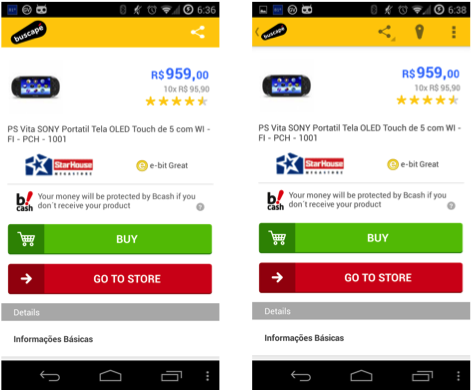
\includegraphics{figures/design-pattern-changes/upnav}
	\caption{Two versions of an app titled ``Buscape'' before (left) and after (right) adopting the Up Navigation pattern. The Up navigation button is shown at the top left corner as a left-facing caret next to the app icon.}
	\label{fig:fig_upnav}
\end{figure}
shows an example of an app before and after using it.

\subsubsection{Discussion}
The Up navigation pattern is less common than navigating with a physical back button. Only 18\% of the apps adopt this pattern. 
The reason behind the Up navigation pattern's low adoption rate could be that apps have relied on the back button for navigation since the initial release of Android, which is already implemented by default. 
The Up navigation button was common in apps that have several sibling activities in the hierarchy (e.g., email clients, shopping apps), which may not be the case for most apps.

\subsection{Navigation Drawers}
\subsubsection{Motivation}
Navigation Drawer is a hidden panel that displays the app's main navigation menu. 
It helps users quickly navigate through the structure of the app. 
When the user taps on the top-left app's icon or swipes from the left to the right of the screen, the Navigation Drawer expands to cover part of the screen and shows a list of items.

\subsubsection{Method}
In order to use the Navigation Drawer, developers need to create a layout with a \textit{DrawerLayout} as the root \textit{ViewGroup} element with two children elements. 
The first child is the Layout element that represents the content when the drawer is hidden and the second is the actual drawer that slides in the Navigation Drawer panel. 
We queried the graph database to find apps that have layouts that starts with a \textit{DrawerLayout} element as a root element with two child views.
\subsubsection{Results}
We found 1,183 apps used the Navigation Drawer. 
Among them, 771 (65.2\%) added it for the first time and only 37 (3.1\%) of the apps stopped using this pattern. Figure~\ref{fig:fig_drawer} shows an example of an app before and after using this pattern.
\begin{figure}[!t]
	\centering
	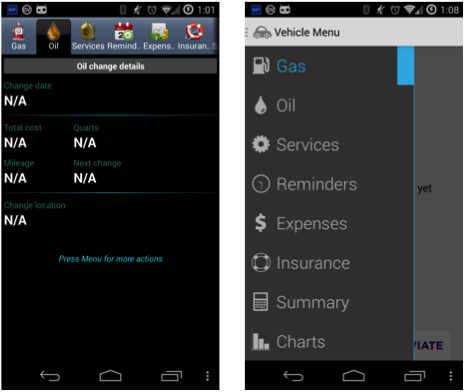
\includegraphics{figures/design-pattern-changes/drawer}
	\caption{Example of an app titled ``Carango - Car Management'' that shows two versions before (left) and after (right) using the Navigation Drawer pattern.}
	\label{fig:fig_drawer}
\end{figure}
\subsubsection{Discussion}
Navigation drawer is relatively less common than other navigation patterns. 
We speculate the reason is two-folds. 
First, implementing this pattern requires a high degree of customization by developers to fit their needs. Second, an app may not have a deep hierarchical navigation structure to make use of this pattern. 
We also found that the majority of the apps using the Navigation Drawer were recent adopters (771 out of 1183), which suggests Navigation Drawer a relatively new design pattern.

\section{Summary}
This chapter presented a large-scale data-mining approach to analyzing design pattern changes.
I discussed its implementation and illustrated a subset of analyses regarding the changes in the use of design patterns (see table~\ref{tab:table_summary}).
This work demonstrated the value of using data-driven approaches to discovering design pattern changes on a large-scale.

\begin{table}[!htbp]
	\def\arraystretch{2}
	\begin{tabular}{| >{\centering\arraybackslash}m{6cm} | m{2cm} | m{2cm} | m{2cm} | m{2cm} |}
		\hline
		\centering \textbf{Design Pattern} & \textbf{Usage} & \textbf{First \ Time} & \textbf{Changes} & \textbf{No Changes} \\
		\hline
		Custom \ UI \ Components & 15,808 & 818 & 410 & 15,398 \tabularnewline
		\hline
		Home Screen Widgets & 2,639 & 255 & 80 & 2,559 \tabularnewline
		\hline
		Resizable Home Screen Widgets & 1,118 & 295 & 24 & 1,094 \tabularnewline
		\hline
		Tab Layout with TabHost & 3,809 & 666 & 413 & 3,396 \tabularnewline
		\hline
		Fragment & 3,963 & 1,814 & 139 & 3,824 \tabularnewline
		\hline
		Horizontal Paging & 4,524 & 941 & 149 & 4,375 \tabularnewline
		\hline
		Action Bar with Tabs & 8,483 & 2,729 & 330 & 8,153 \tabularnewline
		\hline
		Up Navigation & 4,431 & 1,257 & 98 & 4,333 \tabularnewline
		\hline
		Navigation Drawers & 1,183 & 771 & 37 & 11,46 \tabularnewline
		\hline
	\end{tabular}
	\caption{The changes to the presented design patterns. The columns show the name of the design pattern, the number of apps that used this pattern in the dataset, the number of apps that used it for the first time in a recent release, the number of apps that used it but later switched to a different design pattern, and the number of apps that maintained using it in future releases.}
	\label{tab:table_summary}
\end{table}